\subsection{Symbol Decision} \label{sec:symboldecision}

\begin{frame} \frametitle{Symbol Decision}
    \framesubtitle{Phase $\rightarrow$ Symbols}
    \begin{center}
        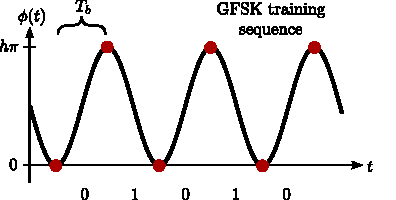
\includegraphics{img/symboldecision}
    \end{center}
    \begin{itemize}
    \item Positive/negative phase change $\Leftrightarrow$ 1/0 symbol.
    \item $T_b = f_s/R = \num{758272}/\num{9600} = \SI{78.987}{samples\per s }$.
    \item From measurement: $T_b = \SI{78.63}{samples\per s}$.
    \item Fractional number of samples:
        \begin{equation*}\tiny
            T_b = [78\ 78\ 80\ 78\ 78\ 80\ 78\ 78\ 80\ 78\ 78\ 80\ 78\ 78\ 80\ 78\ 78\ 80\ 78] \sim 78.63
        \end{equation*}
    \end{itemize}
\end{frame}

\begin{frame} \frametitle{Symbol Decision}
    \framesubtitle{Wrapping Phase $\rightarrow$ Symbols}
    \begin{center}
        \only<1> {
            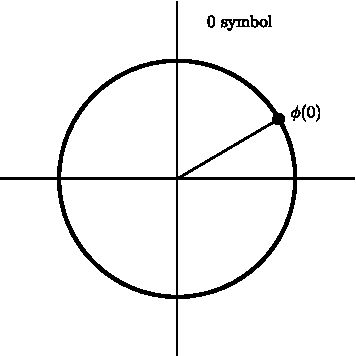
\includegraphics[scale=0.7]{img/symboldecision_animation/0symbol1} \quad
            \includegraphics[scale=0.7]{img/symboldecision_animation/1symbol1}
        }

        \only<2> {
            \includegraphics[scale=0.7]{img/symboldecision_animation/0symbol2} \quad
            \includegraphics[scale=0.7]{img/symboldecision_animation/1symbol2}
        }

        \only<3> {
            \includegraphics[scale=0.7]{img/symboldecision_animation/0symbol3} \quad
            \includegraphics[scale=0.7]{img/symboldecision_animation/1symbol3}
        }
    \end{center}
    \only<1> {
        Wrapped phase at the beginning of a symbol.
    }
    \only<2> {
        Next symbol (for $h=1$): $\phi(0) + \pi = \phi(0) - \pi$.
        \begin{itemize}
        \item The same for 0- and 1-symbol.
        \end{itemize}
    }
    \only<3> {
        Half way to next symbol: Here is a difference!
        \begin{equation*}\footnotesize
            \hat{m}_n = \begin{cases}
                1  &\text{if} \quad \hat{\phi}_{n+0.5} - \hat{\phi}_{n}  >  0\\
                0  &\text{if} \quad \hat{\phi}_{n+0.5} - \hat{\phi}_{n}  <  0\\
                \text{undefined}  & \text{otherwise}
            \end{cases}
        \end{equation*}
        Sync word: Symbol-wise comparison.
    }
\end{frame}

% \begin{frame} \frametitle{Symbol Decision}
%     \framesubtitle{Sync Word and FSM}
%     \begin{center}
%         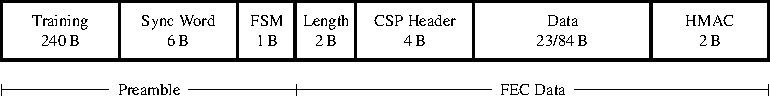
\includegraphics[width=0.9\textwidth]{img/spacelink_format}
%     \end{center}
%     \begin{block}{Sync Word}
%         \begin{itemize}
%         \item End of training sequence -- start of packet.
%         \item Sliding comparison of symbols and sync word.
%         \end{itemize}
%     \end{block}
%     \begin{block}{FSM}
%         \begin{itemize}
%         \item After sync word.
%         \item \texttt{0xA6} $=$ small packet.
%         \item \texttt{0x59} $=$ large packet.
%         \item Else, discard.
%         \end{itemize}
%     \end{block}
% \end{frame}

\begin{frame} \frametitle{Symbol Decision}
    \framesubtitle{Test Results}
    Tested with signal generator.
    \begin{block}{Drifting}
        \begin{itemize}
        \item Little drifting with $T_b\equiv \SI{79}{samples\per s}$.
        \item Correct demodulation of small packet.
        \end{itemize}
    \end{block}
    \begin{block}{With Slope}
        \begin{itemize}
        \item $f_{c,\text{err}} \approx \SI{4000}{Hz}$.
        \item Correct demodulation of small packet.
        \end{itemize}
    \end{block}
    \begin{block}{Finding Sync Word and FSM}
        \begin{itemize}
        \item Sync word $=$ \texttt{OZ4CUB}, FSM $=$ \texttt{0xA6} (small packet).
        \end{itemize}
    \end{block}
\end{frame}

\section{Acceptance Test} \label{sec:finaltest}
\begin{frame} \frametitle{Acceptance Test}
    \framesubtitle{Real-Time Summary}
    \begin{block}{Cycle Count}
        Total number of clock cycles available: \num{142433491}.
        \begin{center}
            \begin{tabular}{|l|r|r|} \hline
                \textbf{Module}         & \textbf{Cycles Used} & \textbf{DSP Usage} \\ \hline
                Sampler                 & \num{109263467}      & \SI{77}{\%}  \\
                Channel Filter          & \num{295467922}      & \SI{207}{\%} \\
                Packet Detector         & \num{ 26435831}      & \SI{19}{\%}  \\
                Mid-Frequency Estimator & \num{ 14322454}      & \SI{10}{\%}  \\
                Time Synchronization    & \num{ 26638224}      & \SI{19}{\%}  \\
                Symbol Decision         & \num{  4587500}      & \SI{3}{\%}  \\ \hline
                Total                   & \num{476715398}      & \SI{335}{\%} \\ \hline
            \end{tabular}
        \end{center}
        \begin{itemize}
        \item C filter $\rightarrow$ Assembly: \SI{86913124}{clock cycles} $\sim$ \SI{61}{\%}.
        \item Downsample complex signal.
        \item Move data when it is processed.
        \end{itemize}
    \end{block}
\end{frame}

\begin{frame} \frametitle{Acceptance Test}
    \framesubtitle{Packet From AAUSAT3}
    \only<1>{
        \begin{block}{Signals}
            \begin{itemize}
            \item Strong, medium, weak.
            \end{itemize}
        \end{block}
        \begin{block}{Criteria}
            \begin{itemize}
            \item Correct sync word and FSM.
            \item Cannot check symbol-by-symbol.
            \end{itemize}
        \end{block}
        \begin{block}{Results}
            \begin{description}
            \item[Strong] Found sync word and FSM.
            \item[Medium] Found sync word and FSM.
            \item[Weak] Wrong sync word -- found later in buffer.
            \end{description}
        \end{block}
    }
    \only<2>{
        \begin{center}
            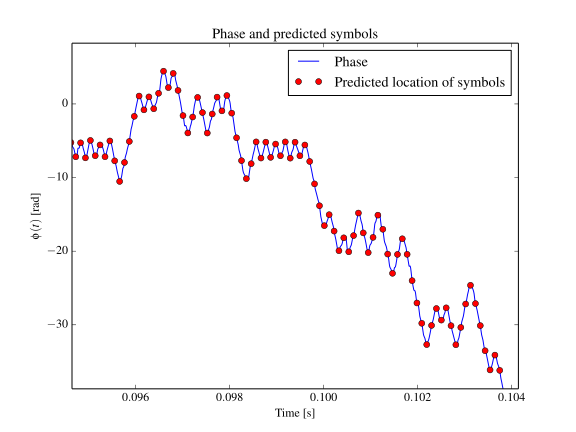
\includegraphics[width=0.7\linewidth]{img/phase_zoom_start_medium}
        \end{center}
        \begin{itemize}
        \item Medium signal.
        \item Sampled $I$ and $Q$ $+$ estimated $f_c$ $\rightarrow$ \textcolor{blue!80!black}{Phase}.
        \item Time synchronized $+$ variable $T_b$ $\rightarrow$ \textcolor{red!80!black}{Predicted location of symbols}.
        \item No drifting -- correct sync word and FSM.
        \end{itemize}
    }
    \only<3>{
        \begin{center}
            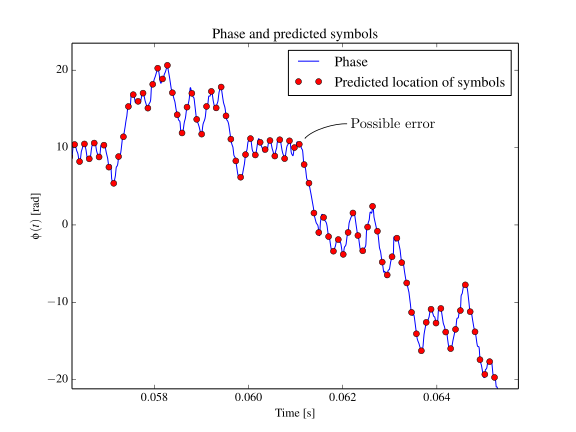
\includegraphics[width=0.7\linewidth]{img/phase_zoom_start_weak}
        \end{center}
        \begin{itemize}
        \item Weak signal.
        \item Sampled $I$ and $Q$ $+$ estimated $f_c$ $\rightarrow$ \textcolor{blue!80!black}{Phase}.
        \item Time synchronized $+$ variable $T_b$ $\rightarrow$ \textcolor{red!80!black}{Predicted location of symbols}.
        \item No drifting -- wrong sync word.
        \end{itemize}
    }
\end{frame}


\section{Conclusion} \label{sec:conclusion}
\begin{frame} \frametitle{Conclusion}
    \begin{itemize}
    \item Detect packet from signal generator.
    \item Correctly demodulate recording from AAUSAT3.
    \item Prepared for real-time optimization.
    \end{itemize}
\end{frame}


\section{Demonstration} \label{sec:demonstration}
\begin{frame} \frametitle{Demonstration}
    \begin{block}{What is Shown?}
        \begin{itemize}
        \item Medium signal strength.
        \item Demodulation on DSP.
        \item Amplitude, spectrogram, FFT (training).
        \item Interactive phase $+$ decisions.
        \end{itemize}
    \end{block}
    \only<1>{
        \begin{center}
            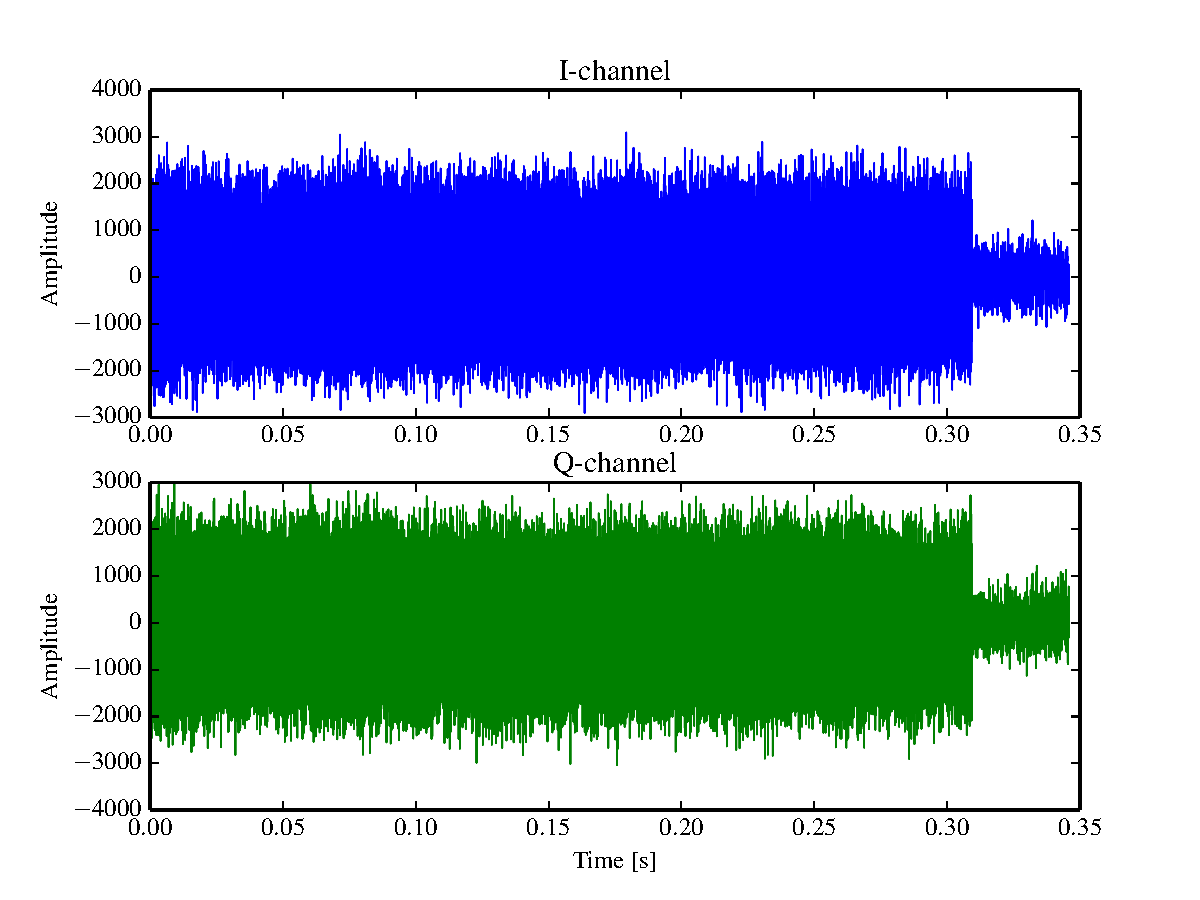
\includegraphics[width=0.6\linewidth]{img/amplitude_zoom_medium}
        \end{center}
    }
    \only<2>{
        \begin{center}
            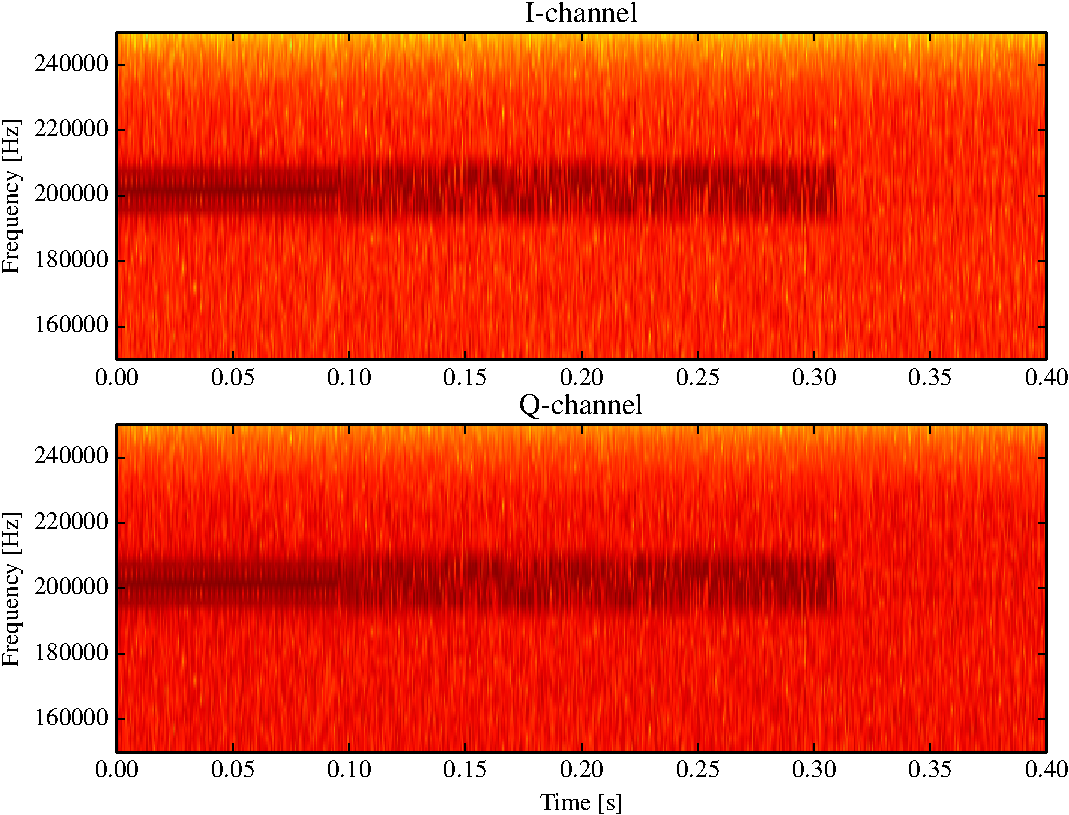
\includegraphics[width=0.5\linewidth]{img/specgram_nofilter_zoom_medium}
        \end{center}
    }
    \only<3>{
        \begin{center}
            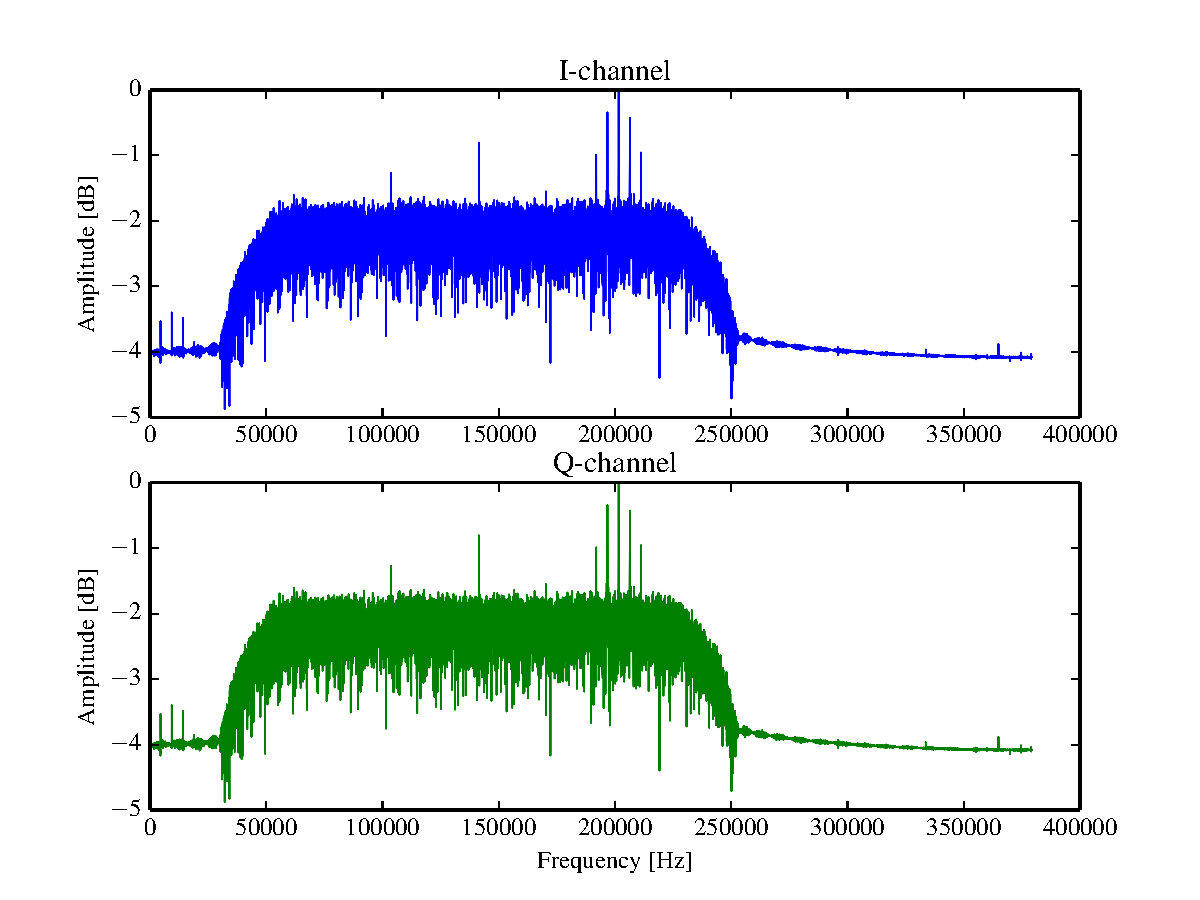
\includegraphics[width=0.6\linewidth]{img/fft_training_nofilter_medium}
        \end{center}
    }
    % \only<1> {
    %     \begin{block}{Output}
    %         \begin{itemize}
    %         \item Plot of phase with predicted symbols (interactive). 
    %         \end{itemize}
    %     \end{block}
    % }
    
\end{frame}

